\begin{frame}
	\frametitle{Random variables}
	A variable quantity whose possible values depend, in random manner, on a set of random outcomes events.\footnote{\href{https://en.wikipedia.org/wiki/Random_variable}{Wikipedia}}\vspace{2em}
	
	Random variables are defined over \emph{probability spaces}: $(\Omega, \mathcal{F}, \mathcal{P})$\\
	Consider a random variable representing the toss of a coin\footnote{Additional information can be found, among others, in \href{http://vfu.bg/en/e-Learning/Math--Bertsekas_Tsitsiklis_Introduction_to_probability.pdf}{D.P. Bertsekas and J.N. Tsitsiklis. "Introduction to Probability"}}
	\begin{itemize}
		\item $\Omega=\{H, T\}$ is the set of possible outcomes. In this case head or tail
		\item $\mathcal{F}=\{\{\}, \{H\}, \{T\}, \{H,T\}\}$ is the set of events we will consider
		\item $\mathcal{P}$ probability function. It associates elements of $\mathcal{F}$ with a probability value. For example $$\mathcal{P}(\{\})=0,\quad\mathcal{P}(\{H\})=0.5, \quad\mathcal{P}(\{T\})=0.5, \quad \mathcal{P}(\{H, T\})=1$$
	\end{itemize}
\end{frame}

\begin{frame}
	\frametitle{Moments}
	For a continuous random variable $X$ taking real values and having probability density function $f(x)$ we can define
	\begin{itemize}
		\item Mean: $E[X]=\int_\mathcal{R} sf(s)ds=\mu$
		\item Variance: second central moment $E[(X-E[X])^2]=\int_\mathcal{R} (s-\mu)^2f(s)ds$
		\item $n$ moment: $n^{th}$ central moment $E[(X-E[X])^n]=\int_\mathcal{R} (s-\mu)^nf(s)ds$
	\end{itemize}
	
	\vspace{1em}
	Not every random variables have all moments of fine moments. For example heavy-tailed distributions:\footnote{\href{https://en.wikipedia.org/wiki/Heavy-tailed_distribution}{\small{ Wikipedia. Heavy-tailed distribution}}} 
	$$f(x)=\left\{\begin{aligned}
					\frac{1}{x^2} && x \geq 1\\
					0&&\textrm{otherwise}
				   \end{aligned}
	\right.$$
\end{frame}

\begin{frame}
	\frametitle{Mean and most likely outcome}
	Mean and the most likely outcome are \emph{different concepts}\vspace{2em}
	
	Consider a discrete random variable $X$ taking values
	\begin{columns}
		\column{0.5\textwidth}
		\begin{itemize}
			\item 0 with probability 0.2 
			\item 1 with probability 0.8
		\end{itemize}
		\vspace*{1em}
	
	    Mean value: $0.2\cdot 0 + 0.8 \cdot 1=0.8$\vspace{0.5em}
	    
		Most likely outcome: $\displaystyle \argmax_{x\in{0,1}} p(x) \;=1$
		
		\column{0.4\textwidth}
		\begin{block}{Probability mass function of $X$}
			\centering
			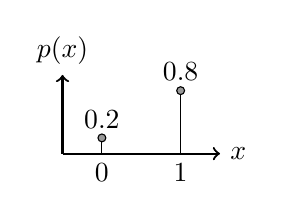
\begin{tikzpicture}
			%\draw[help lines, color=gray!30, dashed] (-4.9,-4.9) grid (4.9,4.9);
			\draw[->, thick] (-0.5,0)--(1.5,0) node[right]{$x$};
			\draw[->, thick] (-0.5,0)--(-0.5,1) node[above]{$p(x)$};
			\draw (0, 0) -- (0, 0.2) node [above] {$0.2$};
			\draw (1, 0) -- (1, 0.8) node [above] {$0.8$};
			\node [below] at (0,0) {0};
			\node [below] at (1,0) {1};
			\filldraw[fill=black!40, draw=black](0,0.2) circle (0.05cm);
			\filldraw[fill=black!40, draw=black](1,0.8) circle (0.05cm);
			\end{tikzpicture}
		\end{block}
	\end{columns}
	
	
	%Under certain assumptions (e.g., Ergodicity) the average of 
	
	\takeaway{The mean value is not even an element of the possible outcomes}
\end{frame}
\begin{frame}
	\frametitle{Sum of independent random variable}
	\onslide<1->The distribution of the sum of two random variables must always be carefully computed\vspace{0.5em}
	\begin{columns}\onslide<1->
		\column{0.5\textwidth}
		\begin{itemize}
			\item <1->$X$ uniform distributed between 0 and 1
			\item <1->$Y$ uniform distributed between 0 and 1
			\item <1->$Z=X+Y$ \emph{is not} uniform distributed between 0 and 1
			\item <2-> The distribution of $Z$ depends on the joint distribution of $X$ and $Y$
			\item <3-> If $X$ and $Y$ are independent variables, then $Z$ has a triangular distribution\\
			for all $x$  in $[0,1]$ and $y$ in [0,1] $$P(X=x,Y=y)=P(X=x)\cdot P(Y=y)$$
			
		\end{itemize}
	
		\column{0.5\textwidth}
		\begin{block}{Probability distributions}
			\onslide<1->{
			\begin{tikzpicture}
				\draw[->] (-0.5,0)--(1.5,0) node[right]{$x$};
				\draw[->] (-0.5,0)--(-0.5,1.5) node[above]{$p(x)$};
				\draw[very thin, dashed] (-0.5, 1)node[left] {1} -- (0, 1);
				\draw[thin](0, 0) node[below] {0}-- (0, 1);
				\draw[thick] (0, 1) -- (1, 1); 
				\draw[thin] (1, 0)node[below] {1} -- (1, 1);
			\end{tikzpicture}}
			\onslide<3->{
			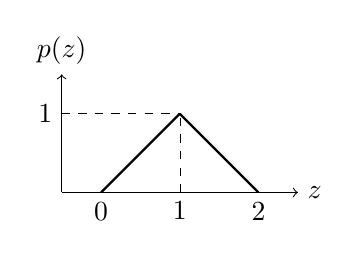
\begin{tikzpicture}
			\draw[->] (-0.5,0)--(2.5,0) node[right]{$z$};
			\draw[->] (-0.5,0)--(-0.5,1.5) node[above]{$p(z)$};
			\draw[very thin, dashed] (-0.5, 1)node[left] {1} -- (1, 1);
			\draw[thick](0, 0) node[below] {0}-- (1, 1);
			\draw[very thin, dashed] (1, 0)node[below]{1} -- (1, 1); 
			\draw[thick] (2, 0)node[below] {2} -- (1, 1);
			\end{tikzpicture}}
		\end{block}
	\end{columns}
\end{frame}
\begin{frame}
	\frametitle{The gaussian/normal distribution $\mathcal{N}$}
	The sum of gaussian distributed random variables \emph{is gaussian distributed}
	\begin{itemize}
		\item $X$ and $Y$ are normally distributed with mean $\mu_x$ and $\mu_y$ and standard deviation $\sigma_x$, $\sigma_y$
		\item $Z=X+Y$ is also normal distributed. Mean: $\mu_z=\mu_x+\mu_y$
		\item <2-> If $X$ and $Y$ are independent, then $\sigma_z=\sqrt{\sigma_x^2 + \sigma_y^2}$
		\item <3-> If $\alpha$ is a non-zero constant, then $\alpha Z$ is normally distributed
		\begin{itemize}
			\item mean is $\alpha \mu_z$
			\item standard deviation is $\alpha \sigma_z$
		\end{itemize}
	
		\item <4-> If $Z$ is a vector of jointly-distributed random variables with mean $\bm{\mu}_z$ and covariance $L=E[(Z-\bm{\mu}_z)(Z-\bm{\mu}_z)^T]$
		and $A$ is a matrix, then
		\begin{itemize}
			\item mean of $AZ$ is $A \mu_z$
			\item covariance matrix of $AZ$ is $ALA^T$
		\end{itemize}
	\end{itemize} 
\onslide<4->{
\takeaway{Note however that $X\cdot Y$ is \emph{not} normally distributed}}
\end{frame}
\begin{frame}
	\frametitle{Gaussian distributions and linear systems}
	Assume 
	\begin{columns}
		\column{0.6\textwidth}
		\begin{itemize}
			\item $X(0)$ is normal distributed $X(0)~\mathcal{N}(\mu_0, \sigma_0^2)$
			\item $W(k)$ is normal distributed $W(k)~\mathcal{N}(\mu_{w,k}, \sigma_{w,k}^2)$
			\item $X(0)$ and $W(k)$ are independent for all $k$
			\item for $k\geq0$ we have $X(k+1) =X(k) + W(k)$
		\end{itemize}	
		\column{0.4\textwidth}
		\begin{block}{Graphical representation}
			\begin{tikzpicture}
			\node(X0){$X(0)$};
			\node[above=1em of X0](W0){$W(0)$};
			\node[right=1em of X0](sum1){$+$};
			\node[right=1em of sum1](X1){$X(1)$};
			\node[above=1.2em of X1](W1){$W(1)$};
			\node[right=1em of X1](sum2){$+$};
			\node[right=1em of sum2](X3){$\cdots$};
			\draw[->] (W0) to (sum1);
			\draw[->] (X0) to (sum1);
			\draw[->] (sum1) to (X1);
			\draw[->] (W1) to (sum2);
			\draw[->] (X1) to (sum2);
			\draw[->] (sum2) to (X3);
			\end{tikzpicture}		
		\end{block}
	\end{columns}
	
	\vspace*{0.5em}

	\onslide<2-> What is the distribution of $X(1)$ ?
	\begin{itemize}\onslide<3->
		\item $X(1)$ is Gaussian distributed (sum of two gaussian variables)
		\item Mean $\mu_1=\mu_0+\mu_{w,0}$, variance $\sigma_1^2 = \sigma_0^2 + \sigma_{w,0}^2$
	\end{itemize}

	\vspace*{0.5em}
	\onslide<4-> What is the distribution of $X(k)$ ?
	\begin{itemize}\onslide<4->
		\item $X(k)$ is Gaussian distributed (sum of gaussian variables)
		\item Mean $\mu_k=\mu_0+\sum_{j=0}^{k-1}\mu_{w,j}$, variance $\sigma_k^2=\sigma_0^2 + \sum_{j=0}^{k-1}\sigma_{w,j}^2$
	\end{itemize}
\end{frame}

\begin{frame}
	\frametitle{Non gaussian distributions and linear systems}
	Assume 
	\begin{columns}
		\column{0.6\textwidth}
		\begin{itemize}
			\item $X(0)$ is uniform distributed $X(0)~\mathcal{U}(0, 1)$
			\item $W(k)$ is uniform distributed $W(k)~\mathcal{U}(0, 1)$
			\item $X(0)$ and $W(k)$ are independent for all $k$
			\item for $k\geq0$ we have $X(k+1) =X(k) + W(k)$
		\end{itemize}	
		\column{0.4\textwidth}
		\begin{block}{Graphical representation}
			\begin{tikzpicture}
			\node(X0){$X(0)$};
			\node[above=1em of X0](W0){$W(0)$};
			\node[right=1em of X0](sum1){$+$};
			\node[right=1em of sum1](X1){$X(1)$};
			\node[above=1.2em of X1](W1){$W(1)$};
			\node[right=1em of X1](sum2){$+$};
			\node[right=1em of sum2](X3){$\cdots$};
			\draw[->] (W0) to (sum1);
			\draw[->] (X0) to (sum1);
			\draw[->] (sum1) to (X1);
			\draw[->] (W1) to (sum2);
			\draw[->] (X1) to (sum2);
			\draw[->] (sum2) to (X3);
			\end{tikzpicture}		
		\end{block}
	\end{columns}
	
	\vspace*{0.5em}
	
	\onslide<2-> What is the distribution of $X(1)$ ?
	\begin{itemize}\onslide<3->
		\item $X(1)$ has a triangular distribution
		\item Mean $\mu_1=\mu_0+\mu_{w,0}$, variance $\sigma_1^2 = \sigma_0^2 + \sigma_{w,0}^2$
	\end{itemize}
	
	\vspace*{0.5em}
	\onslide<4-> What is the distribution of $X(k)$ ?
	\begin{itemize}\onslide<4->
		\item The distribution of $X(k)$ depends on the distribution of $X(k-1)$ and of $W(k-1)$
		\item Mean $\mu_k=\mu_0+\sum_{j=0}^{k-1}\mu_{w,j}$, variance $\sigma_k^2=\sigma_0^2 + \sum_{j=0}^{k-1}\sigma_{w,j}^2$
	\end{itemize}
\end{frame}

\begin{frame}
	\frametitle{Gaussian distributions and non linear systems}
	Assume 
	\begin{columns}
		\column{0.6\textwidth}
		\begin{itemize}
			\item $X(0)$ is uniform distributed $X(0)~\mathcal{U}(0, 1)$
			\item $W(k)$ is uniform distributed $W(k)~\mathcal{U}(0, 1)$
			\item $X(0)$ and $W(k)$ are independent for all $k$
			\item for $k\geq0$ we have $X(k+1) =X^2(k) + W(k)$
		\end{itemize}	
		\column{0.4\textwidth}
		\begin{block}{Graphical representation}
			\begin{tikzpicture}
			\node(X0){$X(0)$};
			\node[above=1em of X0](W0){$W(0)$};
			\node[right=1em of X0](sum1){$+$};
			\node[right=1em of sum1](X1){$X(1)$};
			\node[above=1.2em of X1](W1){$W(1)$};
			\node[right=1em of X1](sum2){$+$};
			\node[right=1em of sum2](X3){$\cdots$};
			\draw[->] (W0) to (sum1);
			\draw[->] (X0) to (sum1);
			\draw[->] (sum1) to (X1);
			\draw[->] (W1) to (sum2);
			\draw[->] (X1) to (sum2);
			\draw[->] (sum2) to (X3);
			\end{tikzpicture}		
		\end{block}
	\end{columns}
	
	\vspace*{0.5em}
	
	\onslide<2-> What is the distribution of $X(1)$ ?
	\begin{itemize}\onslide<3->
		\item $X(1)$ is not Gaussian distributed.
		\item Mean $\mu_1=\mu_0^2+\mu_{w,0}$
	\end{itemize}
\end{frame}


\begin{frame}
	\frametitle{Few remarks}
	\begin{itemize}
		\setlength\itemsep{1.5em}
		\item Mean and variance can be computed in closed form in both cases for all $k$
		\item Only in the gaussian case these mean and covariance completely characterize the distribution of $X(k)$ for all $k$
		\item The gaussian distribution is preserved \emph{only} in the case of linear systems
	\end{itemize}  
\end{frame}